%%% This LaTeX source document can be used as the basis for your technical
%%% report. Intentionally stripped and simplified
%%% and commands should be adjusted for your particular paper - title, 
%%% author, citations, equations, etc.
% % Citations/references are in report.bib 

\documentclass[conference]{acmsiggraph}


\usepackage{graphicx}
\usepackage{hyperref}
\graphicspath{{./images/}}
\newcommand{\figuremacroW}[4]{
\begin{figure}[h] %[htbp]
	\centering
	\includegraphics[width=#4\columnwidth]{#1}
	\caption[#2]{\textbf{#2} - #3}
	\label{fig:#1}
\end{figure}
}

\newcommand{\figuremacroF}[4]{
\begin{figure*}[h] % [htbp]
	\centering
	\includegraphics[width=#4\textwidth]{#1}
	\caption[#2]{\textbf{#2} - #3}
	\label{fig:#1}
\end{figure*}
}


\usepackage{lipsum}

\usepackage{xcolor}
\definecolor{lbcolor}{rgb}{0.98,0.98,0.98}
\usepackage{listings}

\lstset{
	escapeinside={/*@}{@*/},
	language=C,
	basicstyle=\fontsize{8.5}{12}\selectfont,
	numbers=left,
	numbersep=2pt,    
	xleftmargin=2pt,
	%numberstyle=\tiny,
	frame=tb,
	%frame=single,
	columns=fullflexible,
	showstringspaces=false,
	tabsize=4,
	keepspaces=true,
	showtabs=false,
	showspaces=false,
	%showstringspaces=true
	backgroundcolor=\color{lbcolor},
	morekeywords={inline,public,class,private,protected,struct},
	captionpos=t,
	lineskip=-0.4em,
	aboveskip=10pt,
	%belowskip=50pt,
	extendedchars=true,
	breaklines=true,
	prebreak = \raisebox{0ex}[0ex][0ex]{\ensuremath{\hookleftarrow}},
	keywordstyle=\color[rgb]{0,0,1},
	commentstyle=\color[rgb]{0.133,0.545,0.133},
	stringstyle=\color[rgb]{0.627,0.126,0.941},
}


\TOGonlineid{45678}
\TOGvolume{0}
\TOGnumber{0}
\TOGarticleDOI{1111111.2222222}
\TOGprojectURL{}
\TOGvideoURL{}
\TOGdataURL{}
\TOGcodeURL{}

\title{Temple on Mars}

\author{Zoe Wall \\\ 40182161@live.napier.ac.uk \\
Edinburgh Napier University \\
Computer Graphics (SET08116)}
\pdfauthor{Zoe Wall}

\keywords{skybox, hierarchy, lighting, OpenGL, GLSL}

\begin{document}
	
\teaser{
	\centering
	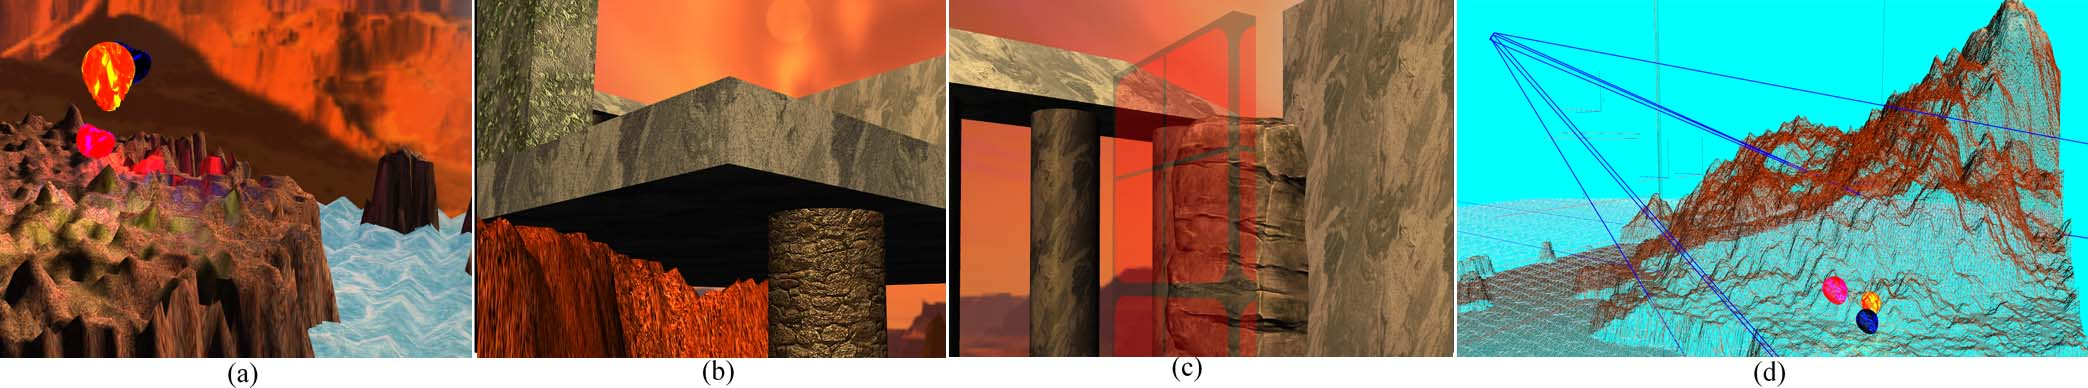
\includegraphics[width=1.0\textwidth]{images/teaser}
	\caption{Project screenshots. (a) Point lights with Vertex Displacement and Parent-Child Hierarchy, (b) Normal Mapping, (c) Transparency and Render Ordering, and (e) View Frustrum Culling and Wireframing.}
	\label{fig:teaser}
}	
	
\maketitle
	
\begin{abstract}
	This project aims to implement a 3D scene, rendered in real-time using OpenGL and C++. The project was intended to be aesthetically interesting, but more importantly intended to show an understanding of fundamental computer graphics principles. This report details the industry techniques used within the development of the outdoor Mars scene.
\end{abstract}
	
\keywordlist
%\copyrightspace
	
\section{Introduction}
	
\figuremacroW
{DestinyMars1}
{Project Inspiration - Destiny Mars Landscape}
{\protect\cite{Destiny}}
{1.0}
	
\paragraph{Project Aims}The main aims of this project were not to produce something photo-realistic but to show understanding of the key concepts of computer graphics. The setting of the scene is a form of landscape on Mars with the inclusion of some extra-terrestrial objects and strange effects. The initial ideas were that of a barren land filled with broken stone and large metallic structures, littered with weeds and with dust clouds. The main inspiration for this type of scene comes from the vast landscapes used within Destiny (see Figure \ref{fig:DestinyMars1}).
	
\paragraph{High Level of Detail} Using different texturing techniques, a high level of detail is hoped to be achieved. For example normal mapping to give the impression of more shape and detail to an object. Along with blend mapping and alpha mapping used on different objects in the scene.
	
\figuremacroW
{fallout}
{Normal Mapping example - Fallout 4}
{\protect\cite{Fallout4}}
{1.0}
	
Even with the improvements to GPU hardware in recent times, there is always a need for optimisation. In this scene optimisation techniques such as a scene graph for spacial partitioning was used alongside view culling.
	
\section{Implementation}

\subsection{Parent-Child Hierarchy}
	
A scene graph in the form of a parent-child hierarchy was implemented within the scene to partition the scene's space into smaller parts to allow for optimization and easier control over the overall development of the scene. The scene graph contains all of the geometry for the particular scene, it makes transformations and rendering easier as a parent-child hierarchy is such that every object in the scene inherits from a single root. This means that each child object's own model matrix is relative to it's parent's (see Listing \ref{lst:hierarchy}).
	
\begin{lstlisting}[label = {lst:hierarchy}, caption={Parent-child Hierarchy Update Method}]
if (parent)
{
	if (parent->myType != sky && myType != sky)
	{
		mworld = parent->mworld * mlocal;
	}
}
	
for (auto &e : children)    // iterate through list of children
{
	Obj* child = e.second;
	child->normalMatrix = normalMatrix;  // set normal matrix for child object 
	child->update(this, delta_time);     // recurse
}
\end{lstlisting}
	
This technique is not only useful for positioning the geometry into world space, it is also useful for rendering and culling. For example, a test can be made to see if an object's parent is not visible within the view frustrum, then it should assume that the child is also not visible and continue without performing the calculations.
Rendering and updating is done by traversing the n-tree that makes up the hierarchy. Firstly the root is rendered if visible. It then iterates through a list of it's children rendering each in turn. If a child of the root is invisible, it will not check to see whether the children are, and the whole branch will be culled. 
	
\subsection{Lighting}
Lighting in computer graphics is very important to get correct as it is the main basis of making a scene look realistic. Lighting calculations are performed on the GPU by programs called shaders. There are three programmable shaders within the graphics pipeline: the vertex, the geometry and the fragment shader.
There are two main methods for lighting a scene using OpenGL: Gouraud shading, and Phong shading.
The Gouraud shading model's calculations are performed per geometry vertex. This means that an object in a scene is coloured by interpolating the colour value between each vertex, as opposed to the more expensive but better Phong shading. Where colour calculations are performed on the fragment shader on a per pixel basis. (See Figure \ref{fig:gouraudPhong})
	
\figuremacroW
{gouraudPhong}
{Implementation of both Gouraud and Phong shading within the project. }
{The sphere on the left is Gouraud shaded, note the specular reflection is less concentrated and accurate, whilst the sphere on the right is Phong shaded.}
{1.0}
	
The main lighting types used within the scene:
\begin{itemize}
	\item {Ambient} Constant lighting which is representative of light from a fixed-intensity and fixed-coloured source. It is used to raise the overall brightness level of every object within the scene. 
	\item {Diffuse} Directional lighting, percentage brightness according to the angle of the light and vertex.
	\item {Specular} Reflective lighting, what makes an object appear to be shiny or reflective.
	\item {Attenuation} Light from a source that degrades over distance such as a point or a spot light.
\end{itemize}
	
The equation for ambient lighting is as follows:
\begin{equation} \label{ambientLightingEq}
	DA
\end{equation}
where $D$ is the diffuse reflection of the material and $A$ is the ambient intensity of the scene. The diffuse reflection is the coloured reflection component of the material.
	
Diffuse lighting is a little more complex as the intensity of the light is not constant. It relies on the direction of the light source to the normal of the geometry. In simple Gouraud shading, the transformed normal of each vertex is calculated, and the angle between that and the light direction is calculated using the scalar product. If the vertex is facing the light source, the intensity of the light will be 100\%, whereas 90 degrees away from the light, the intensity drops to zero.
	
\begin{equation} \label{diffuseLightingEq}
	DA max(L N, 0)
\end{equation}
	
Specular lighting is dependent on the object's material. It is the bright highlight that is dependent on the direction of the eye, in this case the position of the camera. How reflective the material is depends on how bright and how large this highlight appears on the object. In computer graphics it is a very important element in creating a realistic lighting model, as it mimics the reflective properties of a surface. %% reorder
For this calculation, the position of the eye (or camera) must also be taken into account. 
	
\begin{equation} \label{spec}
	SC max(H N, 0)^m
\end{equation}
	
where:
	
\begin{equation} 
	V = \frac{eyePosition - worldPosition}{||eyePosition - worldPosition||}
\end{equation}
	
V is the view direction, where the eye position is the position of the camera, and the world position is the position of the vertex in world space. H from equation \ref{spec} is the half vector, which equates to the view direction plus the direction of the light normalised.

Attenuation lighting is where the lighting is taken from a point source or a spot source, where the intensity is multiplied by a factor of its range. In the real world lighting model, light from a point source drops off exponentially, however attenuation values are set for artistic purposes, to give a more even fall off. 
	
\subsection{Texturing}

\subsubsection{Vertex Displacement}
	
%% jereome
%%Textures used for vertex displacement 
"Vertex Displacement Mapping or simply Displacement Mapping is a technique allowing to deform a polygonal mesh using a texture (displacement map) in order to add surface detail." \cite{Guinot} The scene includes several different methods of vertex displacement including; a procedurally generated terrain from a height map; vertex displacement from a sine wave and scrolling texture for the water effect; and vertex displacement from a displacement map used for the point light's animation.

To generate the terrain for the scene, a height map was used to displace the vertices of the mesh along the y-axis. For extra optimisation the terrain was split into four sections, and the geometry within each quadrant was added to the corresponding section's hierarchy, this is a type of spatial partitioning similar to a quad-tree. The textures were applied using weighting calculations in the y-axis to give the impression of separate parts of the terrain, for example the lowest weight a pebble texture was used for underneath the water.

	
\subsubsection{Normal Mapping}
Normal mapping within the scene is used to give the impression of a greater level of detail to a piece of geometry without the need to render and displace more vertices. The pillars used for the example are uniform cylinders, but using a normal map texture, the lighting calculations can be altered to give the impression of bumps within the shapes.  

\figuremacroW
{normalMap}
{Normal Mapping Example from Scene}
{These pillars are completely smooth cylinder objects, however note how by using a normal map, another level of detail is added making it appear that the pillars are made from stone, with cracks and bumps.}
{1.0}
	
\subsubsection{Skybox}
A skybox is essentially a set of textures called a cube map. These are seamless textures that are laid out in a cube net, which when mapped to the geometry the edges of the cube are not visible. The geometry for the skybox is a cube shape but rendered from the inside out as the renderer culls the inside faces of the shape for optimization. It is scaled and the depth buffer is turned off, by transforming along with the camera's movements this gives the impression that it is infinitely large and far away.
	
\subsubsection{Transparency}
	
To render a transparent object, OpenGL has a mechanism called blending, which combines any colour already in the frame buffer with the colour of the primitive, and the resulting blended colour is stored back in the frame buffer \cite{openGLBlend}. This causes problems for rendering a scene in real-time as render order must be taken into account. This is because if the transparent object is rendered first, the texture behind the object is blended to it, which means that any object rendered after the glass will be occluded by the object.
To solve this issue, an enumeration was used to check for object type when rendering. If the object rendered is a glass object it is rendered separately after the main render function.
	
\section{Post-Processing}
	
%% add definition of post processing here
Post-processing is defined as any rendering technique that is applied after the initial render. These techniques therefore require multiple render passes to different targets. For displaying to the screen, a vertex buffer object is created to use as a render target for the first pass; the scene is rendered normally to this frame buffer then the render target is set back to the screen. For the second render pass, a post process can be applied using the output from the first pass as a texture which is mapped to a screen quad.
	
\subsection{Greyscale}
	
For a grey scale effect, the colour is sampled from a texture of the first render pass. The final colour output is calculated by the dot product of the sampled colour and a greyscale intensity value.
	
\figuremacroW
{greyscale}
{A screen capture of the scene rendering in greyscale}
{This is rendered as a black and white texture mapped to a screen quad.}
{1.0}
	
\subsection{Vignette}
	
A vignette is a loss in clarity and brightness towards the corners of the screen. This effect was created by calculating a radial black and white gradient. The product of this gradient factor and the sampled colour from the original render pass resulted in an output with darker edges. The gradient was achieved by calculating the length of a vector from the screen quad's centre position to the current fragment position, this length was inverted and used as a factor to scale the sampled colour. 
	
\begin{lstlisting}[label = {lst:vignette}, caption={Fragment Shader Code Snippet for Vignette Calculation}]
void main()
{
	// Sample texture colour
	vec4 colourSample = texture(tex, tex_coord);
	
	// calculate the position vector for current pixel
	vec2 position = (gl_FragCoord.xy / resolution) - vec2(0.5);
	
	// get factor
	float len = length(position);
	len = 1.0 - len;
	
	colourSample *= len; // multiply output by inverted length
	
	colour = vec4(colourSample.rgb, 1.0);
}
\end{lstlisting}
	
To calculate the position vector, gl\_FragCoord was used, a built in feature of the pipeline which returns the (x,y) coordinates of the current pixel. This is then divided by the screen's resolution to return a value between 0.0 and 1.0. As gl\_FragCoord uses a lower left origin, to find the centre position (0.5, 0.5) must be subtracted from this total vector.

The length is inverted due to the RGB colour model being additive, meaning that a value of zero for each component will result in black, the shortest lengths are the coordinates closer to the centre of the screen, however multiplying a smaller number to the sampled colour would have produced the opposite effect.
	
\subsection{Shadows}

Shadowing is an important technique to add in any scene to make the lighting model look more realistic. To create a shadow effect, the first render pass of the scene uses the light source's direction and position to render a shadow-map from the point of view of the light that is casting the shadows. A shadow-map is a texture that is taken from the depth buffer of the first render pass see Figure \ref{fig:shadowMap}. It is then used in the second render pass to determine what fragments are in shade. The calculation requires the texture coordinates to be transformed by the light's screen space coordinates. The depth texture is then sampled using these.

\figuremacroW
{shadowMap}
{Shadow Map Example from Scene}
{Here the brightness has been reduced to see more clearly. The shadow map captured from the first render pass, shows the depth of any objects within the field of view of the light source. The darker an object is the closer it is to the light source.}
{1.0}

The resulting x element of the sample is used to determine the shade factor. If the sample is larger than the z component of the projected coordinates in the light's screen space, then the shade factor is set to 0.5. Otherwise the factor remains 1, leaving any fragment not in shade unaltered by the calculation. The final output colour from the fragment shader is the diffuse and specular lighting values scaled by the calculated shade factor. The ambient component of the colour is not scaled as it is supposed to represent a constant overall illumination.

An issue faced when rendering shadows was that of the directional and point lights within the scene. To render shadows, the depth buffer must be captured from the point of view of the light source, however the main directional light is a representation of a sun, where the distance from the light to the scene is infinitely large and therefore the light is approximated to be that it has a constant direction but no position. As for the point light, it emits light in every direction, so the shadow map would have to be in the form of a cube map, to account for the shadows cast in every direction. The scene would have had to be rendered in all 6 different directions and a cube map be rendered. For future work, the shadows could be extended to be more realistic by taking into account these multiple light sources and the different way of rendering them.
	
\subsection{Blur}

A Gaussian blur was implemented within the scene applied in two passes - horizontally and vertically. In the first render pass all of the objects are rendered into a texture, then in the next pass the surrounding horizontal fragments are sampled and combined using pre-defined Gaussian weights. \cite{blurExample} Finally a third render pass is made using the same blur shader, but sampling the surrounding vertical fragments which is rendered to the screen. This has the exact same result as blurring in one render pass but reduces the number of calculations required. Blurring is useful as it can be used in conjunction with other post-processing effects such as Bloom.

\figuremacroW
{bloom_gaussian_two_pass}
{A diagram to show the two-step Gaussian blur sample technique}
{The blur is applied using two render passes to reduce the number of samples needed from a texture. On the left a normal Gaussian blur is shown, but requires a larger number of samples. By blurring in two steps, the exact same effect can be achieved only using 9 samples for each pass. \cite{blurDiagram}}
{1.0}
	
\subsection{Bloom}

Bloom is a technique used for giving the viewer visual cues for the brightness and intensity of a light. Bright lights are usually hard to depict on a screen due to the limited range of intensities of monitors. Bloom is an effect to heighten the perception of bright objects within a scene. There are many different ways to achieve this effect, however the effect within this project was accomplished by rendering two different frame buffers. During the first render pass, all of the objects were rendered normally to a buffer to contain the regular image. Next, this buffer's frame was sampled as a texture and the perceived brightness for each fragment was calculated using the relative luminance equation, see Equation \ref{luma}.

\begin{equation} \label{luma}
Y = 0.2126 R + 0.7152 G + 0.0722 B
\end{equation}

Where Y is the relative luminance: the scalar product of the sampled colour and the luminance values. This is calculated and if it is above a certain threshold, 0.9, the fragment's outgoing colour is set. Otherwise all other fragments are set to black.

This second frame buffer, storing the black or bright parts of the scene is then sent through the Gaussian blur effect, before being rendered finally to the screen. The final render pass takes the output from the two-step Gaussian blur and the output from the initial render pass and sums the sampled colours.


\section{Advanced Rendering Techniques}
	
\subsection{Graphical User Interface}
A GUI was implemented for easier control over the post processing effects, and for frame-rate monitoring. The GUI used within the project was a third-party open source library called ImGui. \cite{imgui} It was simple to integrate into the project and allowed easy functionality for user interaction to save keyboard shortcuts. 
	
\subsection{Particles}

For the particle effect the geometry shader is used in conjunction with transform feedback. A transform feedback is a technique used to capture geometry data before it is rendered. The primitives passed to the geometry shader are first transformed and saved to the transform feedback buffer. This buffer is then used in the second render pass, to output the particles to the screen. Within this project, the second render pass also utilises the geometry shader using a technique called billboarding.

\figuremacroW
{billboards}
{Screen Capture of Smoke Effect}
{This effect uses a transform feedback buffer and a billboarding technique to render the texture facing the user.}
{1.0}

Billboarding is a technique which allows a texture to be rendered always in the direction facing the user. This was used within the second render pass of the particles to render a smoke texture to each, seen in Figure \ref{fig:billboards}.
 
	
\subsection{Optimization}
	
\subsubsection{Profiling}
Originally, with no optimisation techniques implemented, running the performance profiler within Visual Studio 2013 showed that the most expensive call path based on the sample counts was the render() function called to traverse down the hierarchy and render each object in turn.
	
\figuremacroW	
{compare}
{Comparison of Profiling Results}
{The results on the left are after optimization, it shows the hot path render() to be roughly 20\% lower than the original results.}
{1.0}
	
The rendering function initially used 83.20\% of inclusive samples, meaning it was the most expensive function overall. After applying the optimisation techniques, the profiler returned 63.9\% for the main render function meaning the frustrum culling saved on average 20\% of the program's performance. This can also be noted when monitoring the frame-rate for the scene, with the frame-rate clipped, the frame-rate stays at a constant 60FPS. Features such as exploring the environment, and toggling wire-frames on and off make no impact on this frame-rate whatsoever. When running without a clip, the frame rate can be seen to improve when looking away from a complex part of the scene which shows that the view clipping is working, as there is less operations per frame and therefore an improved frame-rate. The slowest parts of the code apart from the render function are part of the geometry builder in the setup of the scene. There is a peak at the start of the program of CPU usage. Further analysis shows that the the hot paths here are both the function to generate the terrain, and the function generating the plane for the water mesh. In both cases, the functions are expensive due to the high number of polygons required to make the mesh look realistic. 
	
	
\subsubsection{Geometry Shader For Debugging}
%%calculate bounding sphere %%show radius algorthim here
The geometry shader is the second part of the graphics pipeline. Unlike the vertex or fragment shaders, the geometry shader is used to transform the actual geometry of an object. A primitive is passed through the shader, for example a point, and the geometry shader then can either add or remove vertices to change the overall shape of the mesh. In the scene, the geometry shader was used to draw the radius of the bounding spheres for each object in the hierarchy. Each mesh has a selection of positions on the vertex array buffer, to calculate the radius a function iterates through positions to find the largest point of the geometry, the length of this as a float is passed into the geometry shader along with the centre point, and a line is drawn.

\subsection{View Frustum Culling}
View frustum culling is an important optimisation technique which essentially means to remove objects that are out of the view of the camera. By calculating the frustum planes of the camera, intersection tests can be performed to see if an object's bounding volume is visible. Any object that is classified as outside of the view frustum is culled - not rendered.

A geometric approach was taken to extract the planes from the view frustum, this involved determining the eight points defining the corners of the near and far plane, and use these points to define all six planes. \cite{lighthouse} The cross product of these corners are then used to find the normal pointing inwards for each plane. Once the planes have been extracted, the plane equation can be used to determine whether the object is inside or outside of the plane. (See equation \ref{planeEq})

\begin{equation} \label{planeEq}
D = \hat{n}\cdot(x_0-x_i)
\end{equation}

Where $D$ is the signed distance from a point $x_0$ to a plane that contains the point $x_i$. $\hat{n}$ is the normalised plane normal. For the intersection test, this equation is repeated for each plane, if the distance is negative for any plane then the centre point lies outside the frustum. To account for objects that intersect with the plane, the test approximates the point to be within the frustum if the distance is less than the radius of the bounding sphere of the object, see Listing \ref{lst:intersection}.

\begin{lstlisting}[ label ={lst:intersection}, caption={Intersection Test for View Frustum}]
for (int i = 0; i < myScene->planeNormals->length(); ++i) 
{
	// for each plane check if 	intersection occurs
	vec3 pointOnPlane;

	if (i < 3)
	{
		pointOnPlane = myScene->planePoints[ftl];		// first three planes are far, top and left therefore corner is in all three
	}
	else
	{	
		pointOnPlane = myScene->planePoints[nbr];
	}

	vec3 centre = vec3(getWorldPos());

	float d;
	d = dot(myScene->planeNormals[i], centre - pointOnPlane);

	if (d < - getRadius())
	{
		//cout << "CULLING! " << this->myName << endl;
		visible = false;
		break;
	}

}
\end{lstlisting}

In the scene the intersection tests are performed using bounding spheres. The use of bounding spheres as volumes is limited due to the fact most objects within the scene are not spheres, for example the columns will have a very wide radius to account for the height, however they will still be classified as within the frustum if horizontal and within it's length, even though it is not visible. However this is a reasonable enough approximation to use as it is less expensive to compute and still noticeably optimizes the render function.

\figuremacroW
{approxFrustum}
{Diagram of Approximation of View Frustum}
{The figure shows a bounding sphere and a frustum. The diagram on the right shows the approximation used in the calculation. If a sphere intersects within the radius boundary of the frustum plane it will be classified as inside the plane. It can lead to incorrect classifications of objects outside the rounded corner, however it is reasonable enough for this case. \cite{RTR}}
{1.0}

\section{Results}

The main aim of the project was to implement a real-time rendered scene using the OpenGL API, whilst developing an understanding of key concepts of computer graphics programming. The aim for the scene's setting was Mars, to give this impression the lighting and textures used within the scene were all very dim and orange looking. The generated terrain was rocky and bumpy to match this barren landscape. Overall the scene is visually interesting, and depicts a stylised impression of a Martian planet. To improve the overall aesthetics of the scene, models could have been used to create the geometry, but this was out of the scope of the assignment. However as stated, the more important goal for this project was to include many advanced concepts to display a good understanding of the subject, which was achieved to a high standard. 

Normal mapping was used to give a higher level of detail to the scene, this is shown within the pillars, given the impression that they are made of stone. Ideally, to add more detail this effect can be added to every texture that is used within the scene.

Another way of adding a high level of detail to the scene would be the inclusion of Screen Space Ambient Occlusion, to give a more realistic lighting effect taking into account that the geometry in the scene is self-occluding. This would have been a good post-processing effect to use, however due to the limited geometry shapes used in the scene, when attempting to implement this effect it wasn't very clear that anything was happening. By using complex models within the scene to make shapes look more realistic, this effect could be included.

To make the lighting more realistic shadows were implemented from the perspective of the spot light on the platform. Implementation of shadows for every lighting source both directional light and point lights would improve the overall lighting model of the scene.

As for optimization techniques, a reasonable approximation of spheres as bounding volumes was used. However, this can lead to some inaccuracies when frustum culling. To improve this, axis-aligned bounding boxes could be used for the geometry of the scene which would make it more accurate.

Within the scene, the bloom is good however could be improved to give a more accurate colour representation. An alternative method for rendering the bloom post-processing technique would be to use deferred rendering. Deferred rendering consists of splitting the render function into smaller sections, for example first rendering all the geometry of the scene, then rendering the lighting model separately. Bloom could be implemented in this way, using a technique to create a higher dynamic range this would involve outputting a vertex buffer object with two colour buffers, one for the normal colour and one for the HDR colour, the scene's lighting would then be rendered using this.

The semi-transparent objects within the scene were rendered correctly, however it would have been good to include a better lighting model for this by taking into account the refraction and reflection of the light.
	
\section{Conclusion}
In conclusion, the project was a success. The scene was implemented in real-time with usable frame-rates, without any slow-down. It showed many core principles of computer graphics, in particular optimisation techniques with view frustum culling, and texturing effects for more than just basic decoration. Future work will be to further the lighting and optimisation techniques to recreate light more realistically. For example to show how light bends as it passes through a transparent object, and use Screen Space Ambient Occlusion to add a further level of detail.
\bibliographystyle{acmsiggraph}
\bibliography{report}

\clearpage
\section{Appendix}

Below are some screenshots of the final results, a video demonstration can be found here:
\url{https://www.youtube.com/watch?v=EeGMYvXEmrg}

\figuremacroW
{pointl}
{Point Lights with Vertex Displacement Showing parent-child Hierarchy.}
{}
{1.0}

\figuremacroW
{radii}
{Wire-framing and Bounding Volume Radii.}
{}
{1.0}

\figuremacroW
{bloom}
{Comparison of with and without Bloom Effect.}
{}
{1.0}
%%\end{minipage}

\figuremacroW
{vignette}
{Vignette Post-Processing Effect.}
{}
{1.0}

\figuremacroW
{blur}
{A Two-Step Gaussian Blur.}
{}
{1.0}

\figuremacroW
{shadow}
{Shadows cast from spot light.}
{}
{1.0}

\figuremacroW
{trans}
{Transparency and Render Ordering.}
{}
{1.0}

\figuremacroW
{view}
{Rendering of a View Frustum when culling is fixed.}
{}
{1.0}

\figuremacroW
{terrain}
{Generated Terrain and Vertex Displaced Water.}
{}
{1.0}

\figuremacroW
{skyb}
{Multiple Overlay of Skyboxes.}
{}
{1.0}


\end{document}